\section{To‘lqin uzunligi. To‘lqinning tarqalish tezligi}




\begin{enumerate}

\item Mexanik to‘lqinlar bu …
\begin{enumerate}[label=\Alph*)]
\item davriy ravishda takrorlanadigan jarayon.
\item mayatnikning tebranishi.
\item tebranishlarning elastik muhitda tarqalishi.
\item tebranishlarning vakuumda tarqalishi.

\end{enumerate}

\item To‘lqin uzunligi bu …
\begin{enumerate}[label=\Alph*)]
\item bir xil fazalarda tebranadigan nuqtalar orasidagi masofa.
\item bir xil fazalarda tebranadigan bir-biriga eng yaqin nuqtalar orasidagi masofa.
\item qarama-qarshi fazalarda tebranadigan bir-biriga eng yaqin nuqtalar orasidagi masofa.
\item qarama-qarshi fazalarda tebranadigan nuqtalar orasidagi masofa.
\end{enumerate}

\item Mexanik to‘lqinlarning tarqalish tezligi qanday muhitda eng katta bo‘ladi?
\begin{enumerate}[label=\Alph*)]
\item havoda.
\item suvda.
\item qattiq jismda.
\item vakuumda.

\end{enumerate}

\item Ikki muhit chegarasi bo‘ylab qanday mexanik to‘lqinlar tarqaladi?
\begin{enumerate}[label=\Alph*)]
\item ko‘ndalang.
\item bo‘ylama.
\item ikki muhit chegarasi bo‘ylab mexanik.
\item hech qanday to‘lqin tarqala olmaydi.

\end{enumerate}

\item Bo‘ylama to‘lqinda muhit zarrachalari qanday yo‘nalishda tebranadilar?
\begin{enumerate}[label=\Alph*)]
\item hamma yo‘nalishlarda.
\item to‘lqin tarqalishiga perpendikular yo‘nalishda.
\item faqat to‘lqin tarqalishi yo‘nalishida.
\item to‘lqin tarqalishi va unga perpendikular yo‘nalishlarda.

\end{enumerate}

\item Ko‘ndalang to‘lqinda muhit zarrachalari qanday yo‘nalishda tebranadilar?
\begin{enumerate}[label=\Alph*)]
\item hamma yo‘nalishlarda.
\item to‘lqin tarqalishiga perpendikular yo‘nalishda.
\item faqat to‘lqin tarqalishi yo‘nalishida.
\item to‘lqin tarqalishi va unga perpendikular yo‘nalishlarda.

\end{enumerate}

\item Gazlarda qanday mexanik to‘lqinlar tarqaladi?
\begin{enumerate}[label=\Alph*)]
\item ham ko‘ndalang, ham bo‘ylama.
\item ko‘ndalang.
\item bo‘ylama.
\item gazlarda to‘lqinlar tarqalmaydi.

\end{enumerate}

\item Ko‘ndalang mexanik to‘lqinlar qanday muhitlar ichida tarqala oladi: 
1) gaz; 2) suyuqlik; 3) qattiq jism.
\begin{enumerate}[label=\Alph*)]
\item faqat 3.
\item faqat 2.
\item faqat 1.
\item 1 va 2.

\end{enumerate}

\item Rasmda tasvirlangan to‘lqinning uzunligi qaysi raqam bilan ko‘rsatilgan?
\begin{enumerate}[label=\Alph*)]
\item 5
\item 4
\item 3
\item 2

\end{enumerate}

\item Rasmda tasvirlangan to‘lqin uzunligini aniqlang (m).

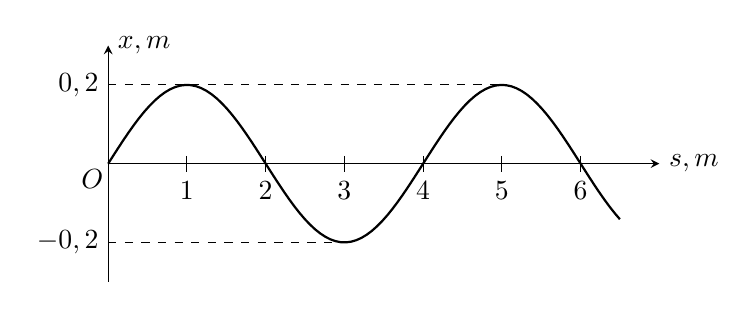
\begin{tikzpicture}[>=stealth]
    % Koordinata o'qlari
    \draw [->] (0,0) -- (7,0) node[right] {$s, m$};
    \draw [->] (0,-1.5) -- (0,1.5) node[right] {$x, m$};
    \node at (-0.2,-0.2) {$O$};

    % To'lqin chizig'i (sinusoida)
    % Masofaga bog'liqlik: peak 1 da, kesishish 2 da, trough 3 da
    \draw [thick, domain=0:6.5, samples=100] plot (\x, {sin(\x*90)});

    % Gorizontal o'qdagi koordinatalar (1 dan 6 gacha)
    \foreach \x in {1,2,3,4,5,6} {
        \draw (\x,0.1) -- (\x,-0.1) node[below] {\x};
    }
    
    % Amplituda qiymatlari va punktir chiziqlar
    \draw [dashed] (0,1) node[left] {$0,2$} -- (5,1);
    \draw [dashed] (0,-1) node[left] {$-0,2$} -- (3,-1);
\end{tikzpicture}

\begin{enumerate}[label=\Alph*)]
\item 5
\item 0,1
\item 4
\item 2

\end{enumerate}

\item Rasmda ko‘ndalang to‘lqinning bir qismi tasvirlangan. Rasmdan foydalanib, to‘lqin uzunligini toping.

\begin{tikzpicture}[>=stealth]
    % Gorizontal o'q (muhit chizig'i)
    \draw (-0.5,0) -- (4,0);
    
    % To'lqin chizig'i (sinusoida)
    % Bu yerda to'lqinning birinchi yarim davri va ikkinchi choragi tasvirlangan
    \draw [thick, domain=0:3.2, samples=150] plot (\x, {2*sin(\x*90)});
    
    % Cho'qqidan (maksimumdan) tushirilgan punktir chiziq
    \draw [dashed] (1,0) -- (1,2);
    
    % To'lqin o'q bilan kesishgan nuqtadan tushirilgan punktir chiziq
    \draw [dashed] (2,0) -- (2,-1);
    
    % 50 cm masofani ko'rsatuvchi ikki tomonlama strelka
    \draw [<->] (1,-0.5) -- node[below, yshift=-2pt] {50 cm} (2,-0.5);
\end{tikzpicture}

\begin{enumerate}[label=\Alph*)]
\item 0,5 m
\item 1 m
\item 2 m
\item 4 m

\end{enumerate}

\item $18$ m oraliqda $4,5$ ta to‘lqin uzunligi joylashsa, bu to‘lqin uzunligi qanday (m)?
\begin{enumerate}[label=\Alph*)]
\item 2
\item 4,5
\item 4
\item 3

\end{enumerate}

\item Elastik muhitda tarqalayotgan to‘lqin, muhit zarrachalari $35$ marta tebrangunga, $70$ m masofani o‘tsa, to‘lqin uzunligi necha metr?
\begin{enumerate}[label=\Alph*)]
\item 0,5
\item 1
\item 2
\item 20

\end{enumerate}

\item Ko‘ndalang to‘lqinning birinchi va beshinchi do‘ngliklari orasidagi masofa 40 m bo‘lsa, to‘lqin uzunligi necha metr bo‘ladi?
\begin{enumerate}[label=\Alph*)]
\item 10
\item 40
\item 4
\item 8

\end{enumerate}

\item To‘lqin uzunligi 3 m bo‘lsa, to‘lqinning uchinchi va yettinchi do‘ngliklari orasidagi masofani toping (m).
\begin{enumerate}[label=\Alph*)]
\item 24
\item 15
\item 18
\item 12

\end{enumerate}

\item Tebranish davri 0,5 s va tarqalish tezligi 20 m/s bo‘lgan to‘lqinning uzunligini toping (m).
\begin{enumerate}[label=\Alph*)]
\item 20
\item 10
\item 4
\item 8
\end{enumerate}

\item Ip (tizimcha) bo‘ylab chastotasi 4 Hz bo‘lgan tebranishlar 8 m/s tezlik bilan tarqalmoqda. To‘lqin uzunligi qanday (m).
\begin{enumerate}[label=\Alph*)]
\item 2
\item 32
\item 4
\item 12

\end{enumerate}

\item Chastotasi 25 Hz va uzunligi 14 m bo‘lgan to‘lqinning tarqalish tezligini toping (m/s).
\begin{enumerate}[label=\Alph*)]
\item 200
\item 350
\item 140
\item 120

\end{enumerate}

\item Tezligi 1800 m/s va uzunligi 20 cm bo‘lgan to‘lqinning chastotasini toping (kHz).
\begin{enumerate}[label=\Alph*)]
\item 12
\item 18
\item 15
\item 9
\end{enumerate}

\item Suv yuzida tarqalayotgan to‘lqin tufayli po‘kak 5 s da 10 marta tebrandi. Agar to‘lqinning ikkita qo‘shni do‘ngligi orasidagi masofa 1 m bo‘lsa, uning tarqalish tezligi qanday (m/s)?
\begin{enumerate}[label=\Alph*)]
\item 2,5
\item 1
\item 2
\item 3
\end{enumerate}

\item Suv sirtidagi to‘lqinning 1- va 3- do‘ngliklari orasidagi masofa 20 cm, uning tarqalish tezligi 0,1 m/s ga teng. To‘lqinning tebranish davrini (s) toping.
\begin{enumerate}[label=\Alph*)]
\item 1,2
\item 0,2
\item 0,5
\item 1
\end{enumerate}

\item Kuzatuvchi dengiz to‘lqinining 2 ta botig‘i orasidagi masofa 12 m ekanligini aniqladi. Agar uning yonidan har 6 s da bitta to‘lqin do‘ngligi o‘tib tursa, to‘lqin tarqalish tezligi necha m/s bo‘ladi?
\begin{enumerate}[label=\Alph*)]
\item 2
\item 4
\item 6
\item 12
\end{enumerate}

\item Suv sirtidagi to‘lqinning 1- va 5- do‘ngliklari orasidagi masofa 20 cm, uning tarqalish tezligi 40 cm/s ga teng. To‘lqinning tebranish davrini (s) toping.
\begin{enumerate}[label=\Alph*)]
\item 0,2
\item 0,5
\item 0,25
\item 0,125
\end{enumerate}

\item Qayiq 1,5 m/s tezlik bilan tarqalayotgan to‘lqin ustida tebranmoqda. To‘lqinning bir-biriga eng yaqin ikki do‘ngligi orasidagi masofa 9 m. Qayiqning tebranishlar davrini toping (s).
\begin{enumerate}[label=\Alph*)]
\item 9
\item 6
\item 4
\item 3

\end{enumerate}

\item Agar ko‘ndalang mexanik to‘lqinlar tarqalayotgan muhitda muhit zarrachalarining tebranishlar amplitudasi 10 cm, maksimal tezligi 30 cm/s ga teng bo‘lsa, to‘lqin tarqalish tezligini aniqlang (m/s). $\lambda = 6\pi$ m.
\begin{enumerate}[label=\Alph*)]
\item 4/3
\item 9
\item 1/6
\item 1

\end{enumerate}

\item Kuzatuvchi sirena tovushini tovush chiqqandan 5 s o‘tgach eshitdi. Agar sirena tovushining chastotasi 2 kHz, to‘lqin uzunligi 15 cm bo‘lsa, u kuzatuvchidan qanday masofada bo‘lgan (m)?
\begin{enumerate}[label=\Alph*)]
\item 100
\item 10000
\item 1500
\item 2000
\end{enumerate}

\item To‘lqinning orasidagi masofa $3\lambda/8$ bo‘lgan ikkita nuqtasining fazalar farqi qanday bo‘ladi?
\begin{enumerate}[label=\Alph*)]
\item $3\pi/4$
\item $2\pi/3$
\item $3\pi/2$
\item $4\pi/3$
\end{enumerate}

\item Koordinatalar boshida joylashgan manbadan to‘lqin uzunligi 2 m bo‘lgan tebranishlar tarqalmoqda. Koordinatalari $x_1=2$ m va $x_2=6$ m bo‘lgan nuqtalarning tebranishlari orasidagi fazalar farqi qanday?
\begin{enumerate}[label=\Alph*)]
\item 0
\item $\pi$
\item $3\pi$
\item $4\pi$
\end{enumerate}

\item Chastotasi 3 Hz bo‘lgan to‘lqin 2,4 m/s tezlik bilan tarqalmoqda. Bir-biridan 20 cm masofada turgan ikki nuqtadagi tebranishlarning fazalar farqi ko‘pi bilan necha radian bo‘ladi?
\begin{enumerate}[label=\Alph*)]
\item $\pi/6$
\item $\pi/4$
\item $\pi/2$
\item $\pi/3$
\end{enumerate}

\item Tebranish davri 0,8 s va tarqalish tezligi 5 m/s bo‘lgan to‘lqinning ikkita nuqtasi orasidagi fazalar farqi $\pi/12$ rad ga teng. Shu ikkita nuqta orasidagi masofa qanday (m)?
\begin{enumerate}[label=\Alph*)]
\item $3/4$
\item $1/24$
\item $2/15$
\item $1/6$
\end{enumerate}

\item To‘lqin tarqalish yo‘nalishi olingan bir to‘g‘ri chiziqda yotuvchi ikki nuqta tebranishlarining fazalari farqi $2\pi$ ga teng. Agar shu nuqtalar orasidagi masofa 2 m bo‘lsa, to‘lqin uzunligi qanday (m)?
\begin{enumerate}[label=\Alph*)]
\item $2\pi$
\item $4\pi$
\item 1
\item 2
\end{enumerate}

\item Ko‘ndalang to‘lqin cho‘zilgan shnur bo‘ylab $v=1,8$ m/s tezlikda $\nu=3$ Hz chastotada tarqaladi. Bir-biridan $\Delta x=0,2$ m masofada joylashgan ikkita nuqta tebranishlarining fazalar farqi nimaga teng?
\begin{enumerate}[label=\Alph*)]
\item $45^\circ$
\item $90^\circ$
\item $120^\circ$
\item $30^\circ$
\end{enumerate}

\item Rasmda tasvirlangan to‘lqinning 0 va 4 nuqtalaridagi fazalar farqi qanday?

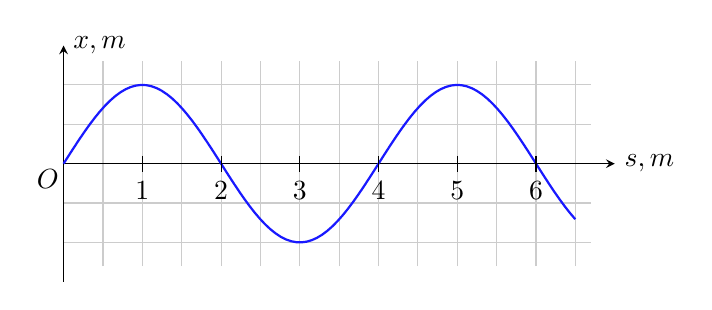
\begin{tikzpicture}[>=stealth]
    \draw[step=0.5cm, gray!40, thin] (0,-1.3) grid (6.7,1.3);
    
    % Koordinata o'qlari
    \draw [->] (0,0) -- (7,0) node[right] {$s, m$};
    \draw [->] (0,-1.5) -- (0,1.5) node[right] {$x, m$};
    \node at (-0.2,-0.2) {$O$};

    % To'lqin chizig'i (sinusoida)
    % Masofaga bog'liqlik: peak 1 da, kesishish 2 da, trough 3 da
    \draw [thick, blue!90, domain=0:6.5, samples=100] plot (\x, {sin(\x*90)});

    % Gorizontal o'qdagi koordinatalar (1 dan 6 gacha)
    \foreach \x in {1,2,3,4,5,6} {
        \draw (\x,0.1) -- (\x,-0.1) node[below] {\x};
    }
           
\end{tikzpicture}

\begin{enumerate}[label=\Alph*)]
\item $\pi/3$
\item $2\pi$
\item $\pi$
\item $\pi/2$
\end{enumerate}

\item X o‘q bo‘ylab tarqaluvchi yassi to‘lqinning qarama-qarshi fazada tebranadigan ikki nuqtasi orasidagi eng kichik masofa 1,6 m bo‘lsa, to‘lqin uzunligi qanday?
\begin{enumerate}[label=\Alph*)]
\item 1,8
\item 3,2
\item 6,4
\item $4\pi$
\end{enumerate}

\item Rasmda to‘lqin tasvirlangan. Keltirilgan javoblardan bir xil fazada tebranayotgan nuqtalarni aniqlang.

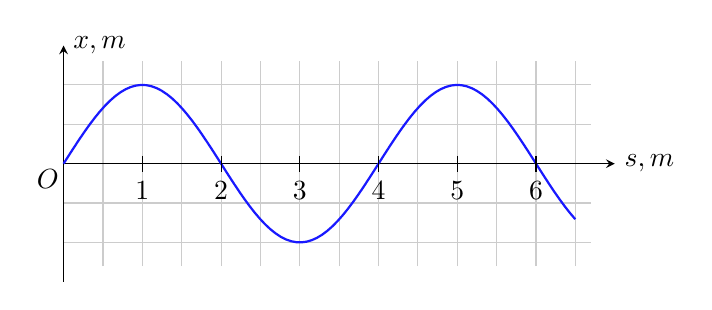
\begin{tikzpicture}[>=stealth]
    \draw[step=0.5cm, gray!40, thin] (0,-1.3) grid (6.7,1.3);
    
    % Koordinata o'qlari
    \draw [->] (0,0) -- (7,0) node[right] {$s, m$};
    \draw [->] (0,-1.5) -- (0,1.5) node[right] {$x, m$};
    \node at (-0.2,-0.2) {$O$};

    % To'lqin chizig'i (sinusoida)
    % Masofaga bog'liqlik: peak 1 da, kesishish 2 da, trough 3 da
    \draw [thick, blue!90, domain=0:6.5, samples=100] plot (\x, {sin(\x*90)});

    % Gorizontal o'qdagi koordinatalar (1 dan 6 gacha)
    \foreach \x in {1,2,3,4,5,6} {
        \draw (\x,0.1) -- (\x,-0.1) node[below] {\x};
    }
           
\end{tikzpicture}

\begin{enumerate}[label=\Alph*)]
\item 2, 4
\item 1, 5
\item 1, 3
\item 3, 5
\end{enumerate}

\item To‘lqin sirti ta’rifini to‘g‘ri mazmunda to‘ldatuvchi javobni aniqlang. To‘lqin sirti deb …
\begin{enumerate}[label=\Alph*)]
\item bir xil fazada tebranuvchi nuqtalarning …
\item bir xil chastota bilan tebranuvchi nuqtalarning …
\item bir xil amplituda bilan tebranuvchi nuqtalarning …
\item tebranish davrlari bir xil bo‘lgan nuqtalarning …
\end{enumerate}

\item Quyidagi rasmda ko‘ndalang to‘lqin tasvirlangan. To‘lqin A dan B nuqtagacha borishi uchun 0,2 s vaqt sarflaydi. To‘lqin chastotasini toping (Hz).

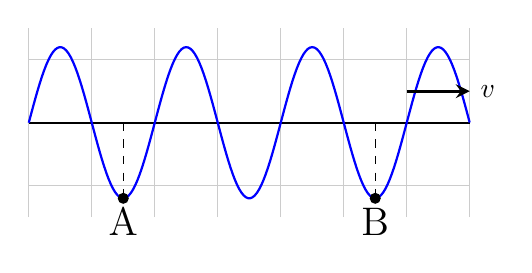
\begin{tikzpicture}[scale=0.8]
    % Katakli fon (setka)
    \draw[step=1cm, gray!40, thin] (0,-1.5) grid (7,1.5);
    
    % Asosiy muvozanat o'qi
    \draw[thick] (0,0) -- (7,0);
    
    % To'lqin chizig'i (Sinusoida)
    % Bu yerda to'lqin uzunligi lambda = 2 katakka teng qilib olingan
    \draw [thick, blue, domain=0:7, samples=200] plot (\x, {1.2*sin(\x*180)});

    % A va B nuqtalarini belgilash (Botiqliklar ostida)
    % A nuqta - birinchi botiqlik ostida (x=1.5)
    \draw[dashed] (1.5, 0) -- (1.5, -1.2);
    \node[below] at (1.5, -1.2) {\Large A};
    \fill (1.5, -1.2) circle (2.5pt);
    
    % B nuqta - uchinchi botiqlik ostida (x=5.5)
    % Har 2 katakda botiqlik takrorlanadi: 1.5 -> 3.5 -> 5.5
    \draw[dashed] (5.5, 0) -- (5.5, -1.2);
    \node[below] at (5.5, -1.2) {\Large B};
    \fill (5.5, -1.2) circle (2.5pt);
    
    % To'lqinning tarqalish yo'nalishini ko'rsatuvchi strelka (ixtiyoriy)
    \draw[->, >=stealth, very thick] (6, 0.5) -- (7, 0.5) node[right] {$v$};
\end{tikzpicture}

\begin{enumerate}[label=\Alph*)]
\item 15
\item 20
\item 5
\item 10
\end{enumerate}

\item Ko‘ndalang to‘lqin o‘ng tomonga tarqalmoqda. A va B nuqtalar qanday yo‘nalishda harakat qiladi?

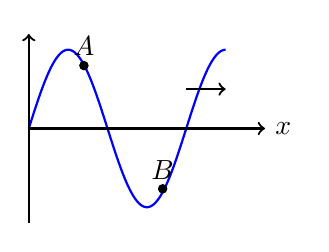
\begin{tikzpicture}
\draw [thick, blue, domain=0:2.5, samples=200] plot (\x, {sin(\x*180)});

\draw[thick,->] (0,0) -- (3,0) node[right] {$x$};
\draw[thick,->] (0,-1.2) -- (0,1.2);
\draw[thick,->] (2,0.5) -- (2.5,0.5);
\coordinate (A) at (0.7, {sin(53)});
    \filldraw (A) circle (1.5pt) node[above] {$A$};

\coordinate (B) at (1.7, {sin(-50)});
    \filldraw (B) circle (1.5pt) node[above] {$B$};

\end{tikzpicture}

\begin{enumerate}[label=\Alph*)]
\item o‘ngga.
\item yuqoriga.
\item A nuqta yuqoriga, B nuqta pastga.
\item A nuqta pastga, B nuqta yuqoriga.
\end{enumerate}

\item Rasmda ko‘rsatilgan ko‘ndalang to‘lqin o‘ng tomonga tarqalmoqda. A va B nuqtalarning harakat yo‘nalish-larini aniqlang.

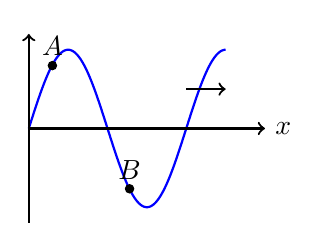
\begin{tikzpicture}
\draw [thick, blue, domain=0:2.5, samples=200] plot (\x, {sin(\x*180)});

\draw[thick,->] (0,0) -- (3,0) node[right] {$x$};
\draw[thick,->] (0,-1.2) -- (0,1.2);
\draw[thick,->] (2,0.5) -- (2.5,0.5);
\coordinate (A) at (0.3, {sin(53)});
    \filldraw (A) circle (1.5pt) node[above] {$A$};

\coordinate (B) at (1.28, {sin(-50)});
    \filldraw (B) circle (1.5pt) node[above] {$B$};

\end{tikzpicture}

\begin{enumerate}[label=\Alph*)]
\item ikkala nuqta o‘ngga.
\item ikkala nuqta pastga.
\item A-nuqta pastga, B-nuqta yuqoriga.
\item A-nuqta yuqoriga, B-nuqta pastga.
\end{enumerate}

\item Turg‘un to‘lqinning qo‘shni tugunlari orasidagi masofa 0,125 m bo‘lsa, to‘lqin uzunligi necha metr bo‘ladi?
\begin{enumerate}[label=\Alph*)]
\item 0,25
\item 0,5
\item 0,75
\item 1
\end{enumerate}

\item Turg‘un to‘lqinning birinchi va yettinchi tugunlari orasidagi masofa 18 cm. To‘lqin uzunligi qanday (cm)?
\begin{enumerate}[label=\Alph*)]
\item 9
\item 18
\item 6
\item 54
\end{enumerate}

\item Birinchi va uchinchi tugunlari orasidagi masofa 0,2 m bo‘lgan turg‘un to‘lqin uzunligini toping (m).
\begin{enumerate}[label=\Alph*)]
\item 1
\item 0,6
\item 0,4
\item 0,2
\end{enumerate}



\end{enumerate}





\begin{center}
\begin{tabular}{|c|c|c|c|c|c|c|c|c|c|}
\hline
1C & 2B & 3C & 4A & 5C & 6B & 7A & 8A & 9B & 10C \\
\hline
11C & 12C & 13C & 14A & 15D & 16B & 17A & 18B & 19D & 20C \\
\hline
21D & 22A & 23D & 24B & 25B & 26C & 27A & 28D & 29C & 30D \\
\hline
31D & 32C & 33B & 34B & 35B & 36A & 37D & 38C & 39C & 40A \\
\hline
41C & 42D & & & & & & & & \\
\hline
\end{tabular}
\end{center}